\documentclass[]{article}

%opening

\usepackage{amsmath}
\usepackage{amsfonts}
\usepackage{float}
\usepackage{hyperref}
\usepackage[explicit]{titlesec}
\usepackage{xcolor}
\usepackage{graphicx}

\title{B\&W Colorising Models\\Project Report 1\\}
\author{
	Ashera Dyussenova\\
	\texttt{a.dyusenova@innopolis.university}
	\and
	Mark Zakharov\\
	\texttt{ma.zakharov@innopolis.university}
	\and
	Nikolay Pavlenko\\
	\texttt{n.pavlenko@innopolis.university}
}
\date{September 2023}

\begin{document}
	
	\maketitle
	
	\section{Project Topic}
	
	After considering various options presented to us, we have decided to select \textbf{A model for colorizing B\&W pictures} as the topic for our course project. We were interested in it because image colorization is a task where advantages of the AI and deep learning over hard-coding are most readily apparent. The task itself is also relevant, as it can be applied from colorization and re-colorization of old film recordings to historical image data, of which no colorized version survived. \\ In our project we intend to develop several ML models, building and evaluating different model architectures and loss functions, with the goal of finding an optimal model for the task at hand. We're particularly interested in implementing generative adversarial networks, as they have shown promising results in the field of image-to-image translation and image colorization.
	
	\section{Project Plan}
	
	We estimate that development, training and evaluation of different model architectures will be the most difficult part of the project, so in our current project plan most of the time is devoted to it in particular:
	
	\begin{itemize}
		\item \textbf{Weeks 3-5}: research into the subject, data gathering, understanding and preprocessing;
		\item \textbf{Weeks 6-11}: development and training of several models, evaluation and recording of the results;
		\item \textbf{Weeks 12-13}: deployment of the models (possibly using Streamlit), evaluation the entire project in the technical report.
	\end{itemize}
	
	\section{Division of Responsibilities}
	
	While our team mostly works collaboratively on different parts of the subtasks encountered in the project, if we were to define different areas of responsibility, we would get the following picture:
	
	\begin{itemize}
		\item \textbf{Ashera Dyussenova}: researcher, model developer, documentation specialist;
		\item \textbf{Mark Zakharov}: data preprocessing specialist, model developer, deployment engineer;
		\item \textbf{Nikolay Pavlenko}: data analyst, model developer, project coordinator.
	\end{itemize}
	
	\section{Current Progress}
	
	\subsection{Datasets Exploration}
	
	In order to head-start our project, we had to find some large enough datasets containing black and white pictures. Two have been chosen so far:
	
	\begin{itemize}
		\item \textbf{Fashion-MNIST} - a dataset comprising of 28×28 grayscale images of 70,000 fashion products from 10 categories, with 7,000 images per category. Could be a useful dataset for image colorization as it maintains the same image size, and has a large number of samples that can be used in training\cite{mnist};
		\item \textbf{Image Colorization} - a dataset that contains 25k 224x224 grayscale and colored images. While it has fewer datapoints than the Fashion-MNIST dataset, its images have better resolution and have colored ones, making it possible to train and test our models on it. This dataset is also a part of a competition on Kaggle, so we can see multiple solutions to our problem, using them as inspiration behind our B\&W translation models.\cite{image_colorization}
	\end{itemize}
	
	To conclude, we will be training and evaluating our models on the second dataset, while using images from the first dataset to test our models at the deployment stage.
	
	\subsection{Describing the Data}
	
	As mentioned prior, we have both grayscale and colored images in the Image Colorization dataset. Those images aren't strictly limited to a single topic, so models developed on this dataset are more generalized than if they had been developed on MNIST dataset:
	\begin{figure}[H]
		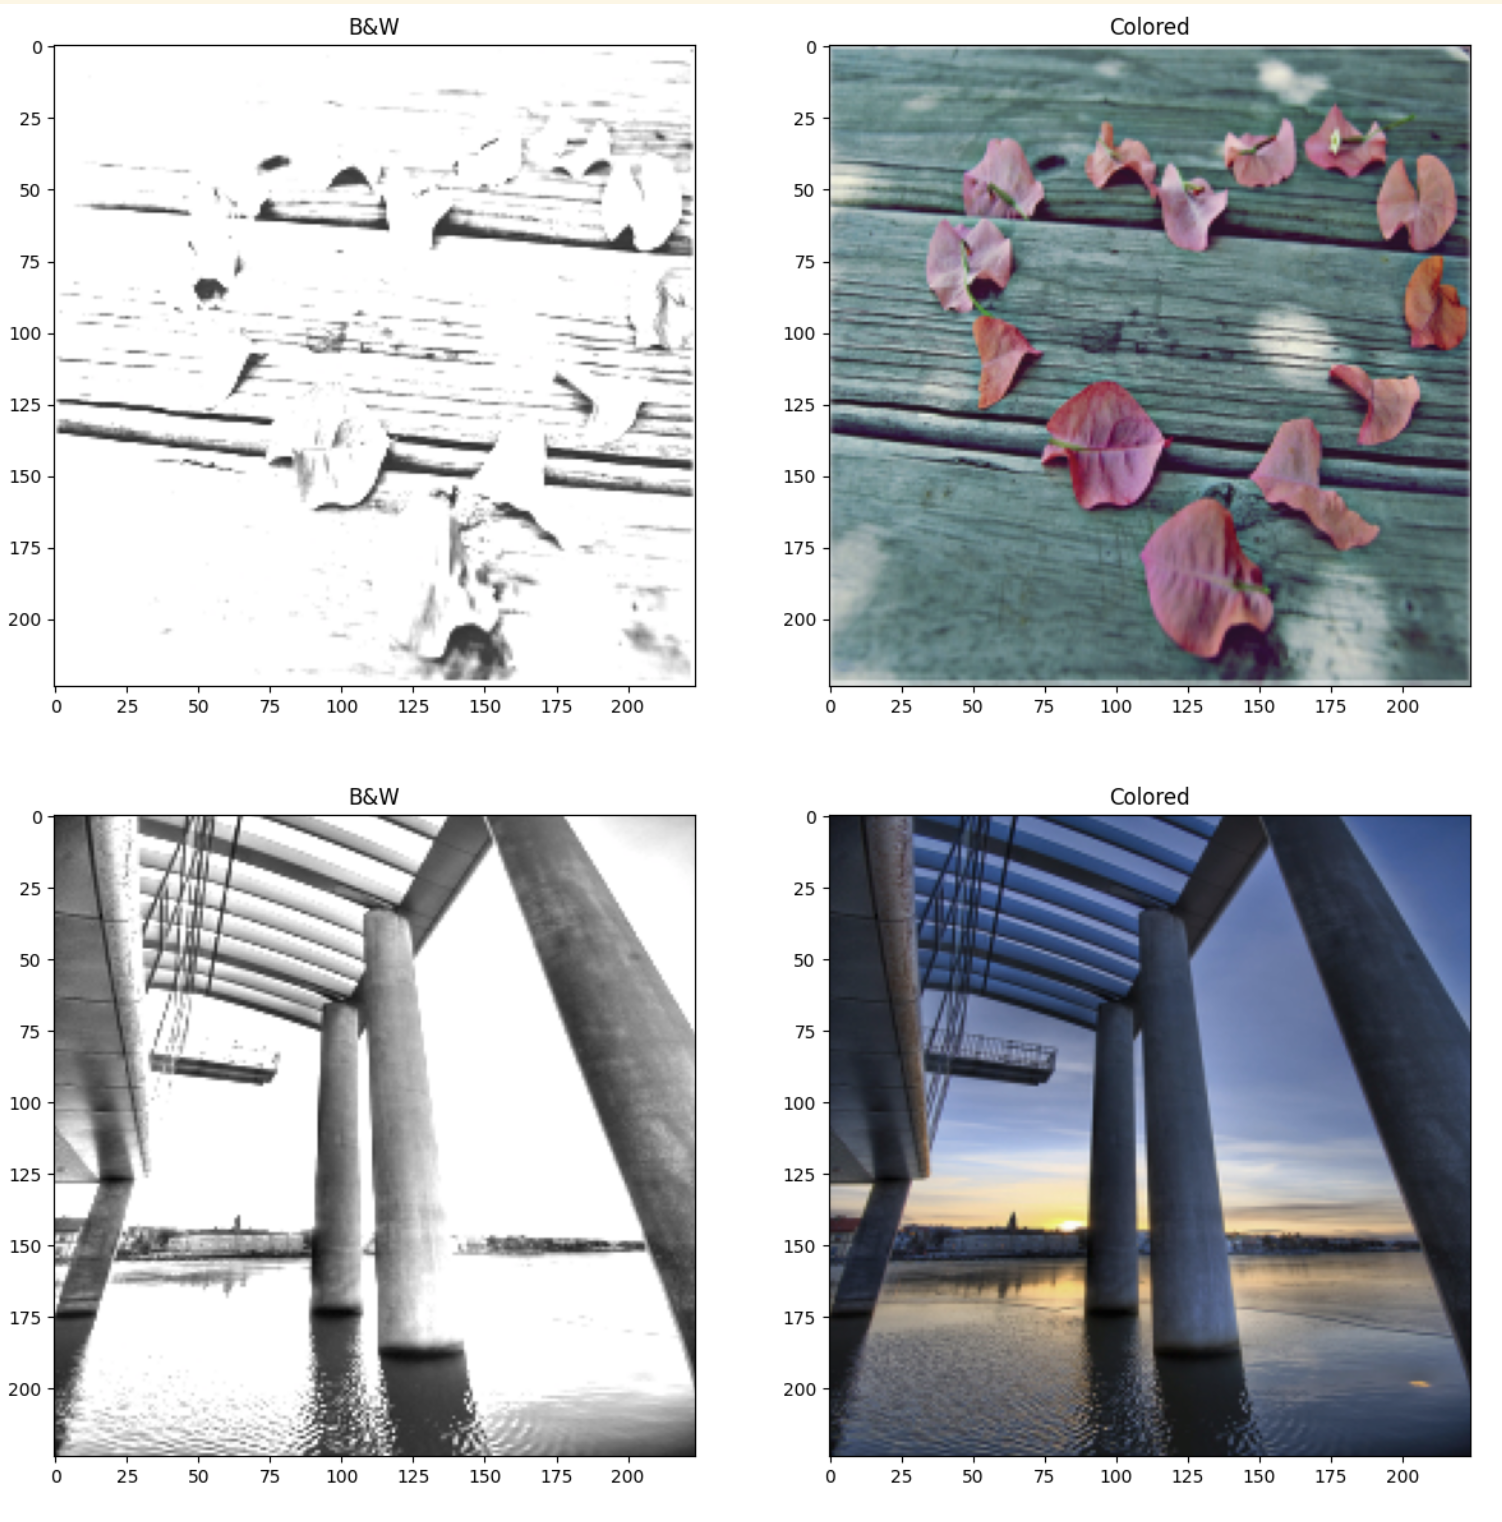
\includegraphics{image1.png}
	\end{figure}
	
	\section{Team Name and Github}
	
	As our team name, we have selected: \textbf{Bokassa}(really should be changed. while naming the team after an African war criminal is funny, it is also too weird for my comfort zone).
	
	\textbf{Link:}\href{https://github.com/Daru1914/B-W-Colorising-Models}{\emph{https://github.com/Daru1914/B-W-Colorising-Models}}
	
	\begin{thebibliography}{9}
		\bibitem{mnist} https://paperswithcode.com/dataset/fashion-mnist
		\bibitem{image_colorization}
		https://www.kaggle.com/datasets/shravankumar9892/image-colorization
	\end{thebibliography}
	
\end{document}
